\chapter{مقدمه}
\label{chap:intro}

‫شبکه‌های بی‌سیم نسل ششم در حال حاضر به عنوان چشم‌انداز آینده ارتباطات مطرح هستند و پیش‌بینی می‌شود که ویژگی‌هایی مانند پوشش گسترده منطقه‌ای، ارائه خدمات متنوع برای سناریوهای پیش‌بینی شده، اتصالات انبوه و ناهمگونی پویا را به همراه داشته باشند. این ویژگی‌های پیشرفته منجر به ایجاد مسائل بهینه‌سازی شبکه در مقیاس بزرگ و پیچیده‌ای می‌شوند. در دهه‌های اخیر، سامانه‌های ارتباطات بی‌سیم ستون فقرات جامعه مدرن بوده‌اند و کاربردهایی از ارتباطات شخصی تا اتوماسیون صنعتی را ممکن ساخته‌اند. با این حال، با رسیدن شبکه‌های نسل پنجم
\lr{(\gls{5G})}
 به بلوغ تجاری، تقاضای فزاینده‌ای برای نرخ داده‌های بسیار بالا و برنامه‌های جدید به وجود آمده است که نیازمند اتصال انبوه هستند (مانند اینترنت اشیا 
\lr{(\gls{IoT})}
  و 
\gls{Metaverse}
  ). این افزایش تقاضا منجر به رقابت فزاینده‌ای برای تخصیص کارآمد طیف می‌شود؛ زیرا شبکه‌های آینده باید حجم عظیمی از داده‌ها را پشتیبانی کنند.‬

‫‬
‫روش‌های مرسوم مبتنی بر مدل با وجود کارآیی در سناریوهای ساده که مدل‌های ریاضی دقیقی برای آن‌ها وجود دارد، در مواجهه با کاربردهای پیچیده و واقعی شبکه‌های نسل ششم، با چالش بار محاسباتی بالا و زمان‌ پردازش طولانی دست و پنجه نرم می‌کنند. به طور موازی، پیشرفت‌های اخیر در یادگیری ماشین و به طور خاص 
\gls{Deep Learning}
، رویکردهای نویدبخشی را برای حل مسائل پیچیده و غیرقابل حل در گذشته را در لایه فیزیکی و مدیریت منابع شبکه ارائه کرده‌اند. روش‌های 
\gls{Deep Learning}
صرفاً مبتنی بر داده توانایی‌های تقریب قدرتمندی را ارائه می‌دهند و می‌توانند استنتاج برخط سریعی داشته باشند. با این حال، محدودیت‌های این روش‌ها شامل نیاز به مجموعه داده‌های ناکافی یا بزرگ و همچنین ضعف در
\gls{Interpretability}
 است. در حوزه هوش مصنوعی، پژوهشگران به دنبال آن هستند که رایانه‌ها بتوانند دانش را مانند انسان درک کنند، به دست آورند، پردازش کنند و استنتاج نمایند. برای این منظور، مهندسی مبتنی بر دانش پیشنهاد شده است، که در آن سامانه‌های خبره برای تقلید از توانایی استدلال انسان ساخته می‌شوند. این مسائل، لزوم حرکت به سمت رویکردهای ترکیبی را نشان می‌دهد که بتوانند از مزایای ساختاریافته مدل‌های ریاضی و انعطاف‌پذیری و سرعت 
\gls{Deep Learning}،
 به طور همزمان استفاده کنند.‬

‫برای رفع چالش‌هایی که مدل‌های مرسوم و روش‌های صرفاً مبتنی بر داده با آن مواجه هستند،
\gls{Knowledge-Driven Deep Learning}
 معرفی شده است. این رویکرد 
\gls{Domain Knowledge}
  را در شبکه‌های عصبی ادغام می‌کند و نقاط قوت هر دو روش مبتنی بر مدل و مبتنی بر داده را ترکیب می‌نماید.
\gls{Knowledge-Driven Deep Learning}
   با هدف ارائه یک راهنمای روشنگر برای ترکیب موثر 
\gls{Domain Knowledge}
    در شبکه‌های عصبی در حوزه ارتباطات بی‌سیم، به دنبال پیشبرد شبکه‌های نسل ششم هوشمند، کارآمد و قابل اعتماد است. در این زمینه، مفهوم دانش دامنه خاص ارتباطات به طور جامع تعریف شده است؛ این دانش شامل نظریه‌های فنی و شناخت تجربی است که توسط دانشمندان و متخصصان در فرآیند تصور، ساخت و بهینه‌سازی شبکه‌های ارتباطی بی‌سیم انباشته شده است. این دانش به دو جنبه کلیدی تقسیم می‌شود. نخست، دانش در طول فرآیند مدل‌سازی مانند مدل‌سازی نظریه‌های وظایف بی‌سیم و دیگری، دانش در طول فرآیند تصمیم‌گیری مانند الگوریتم‌های نظری مبتنی بر مدل. به طور کلی، دانش دامنه در شبکه‌های بی‌سیم به دانش علمی و دانش تخصصی طبقه‌بندی می‌شود که اولی رسمی‌تر و دومین غیررسمی‌تر است. دانش علمی شامل قوانین نظری انتقال، روش‌های مدل‌سازی شبکه‌های بی‌سیم و راه‌حل‌های نظری بهینه‌سازی شبکه است، که اغلب به صورت رابطه‌های ریاضی رسمی بیان می‌شوند.‬
   
‫یکی از قدرتمندترین نمودهای 
\gls{Knowledge-Driven Deep Learning}،
 روش 
\gls{Deep Unfolding}
 است که به طور گسترده در پردازش سیگنال و بهینه‌سازی شبکه‌های بی‌سیم نسل جدید مورد بررسی قرار گرفته است. این روش، الگوریتم‌های تکرارشونده مرسوم مانند روش‌های بهینه‌سازی یا تخمین سیگنال را به صورت لایه‌های ساختاریافته در یک 
\gls{Deep Neural Network}
نگاشت می‌کند. این رویکرد، قابلیت تفسیر 
\gls{Interpretability}
  را با حفظ ساختار اصلی الگوریتم‌های تکرارشونده افزایش می‌دهد، در حالی که پارامترهای الگوریتم‌های مرسوم مانند اندازه‌های گام یا ضرایب همگرایی به 
\glspl{Trainable Parameter}
   در 
\gls{Deep Neural Network}
    تبدیل می‌شوند. این امر امکان استفاده از بهینه‌سازی مبتنی بر داده را فراهم می‌سازد تا همگرایی تسریع شود و عملکرد بهبود یابد. برخلاف 
\gls{post-hoc explainability}   
   که پس از آموزش مدل‌ها اتفاق می‌افتد،
\gls{Knowledge-Driven Deep Learning}
     به نظام فکریِ
\gls{ante-hoc explainability}     
     تعلق دارد که در آن تفسیرپذیری از همان ابتدا در طراحی مدل یا فرآیند یادگیری جاسازی می‌شود. این ویژگی به ویژه در شبکه‌های بی‌سیم که الزامات حیاتی ایمنی دارند مهم است.‬
     
پژوهش‌های انجام شده در منابع نشان می‌دهد که فقدان یک طبقه‌بندی یکپارچه و نظام‌مند از رویکردهای ادغام دانش برای بهینه‌سازی شبکه‌های بی‌سیم، یک شکاف تحقیقاتی مهم بوده است. در پاسخ به این نیاز، یک طبقه‌بندی جدید برای رویکردهای ادغام دانش در شبکه‌های بی‌سیم پیشنهاد شده است که بر اساس این موضوع طراحی شده که دانش دامنه در کدام اجزای 
\gls{Pipeline}
\gls{Deep Learning}
و به چه شکلی ادغام می‌شود. این طبقه‌بندی شامل ادغام دانش دامنه در انتخاب مدل شبکه عصبی، سفارشی‌سازی مدل شبکه عصبی، ساخت معماری ترکیب دانش و داده، طراحی 
\gls{Loss Function}
 و پیکربندی 
\gls{Hyperparameter}
  است. این چارچوب ساختاریافته، یک دستورالعمل عمل برای ادغام دانش و شبکه‌های عصبی ارائه می‌دهد.‬
‫از منظر کاربرد، تمرکز اصلی رویکردهای دانش‌محور و 
\gls{Deep Unfolding}
 در شبکه‌های بی‌سیم بر دو حوزه اساسی تخصیص منابع و پردازش سیگنال است. در حوزه تخصیص منابع، روش‌هایی مانند گسترش الگوریتم 
\gls{WMMSE}
 با استفاده از
\glspl{Graph Neural Network}
 برای تخصیص توان کارآمد و مقیاس‌پذیر مورد استفاده قرار گرفته‌اند. در پردازش سیگنال نیز، 
\gls{Graph Neural Network}
  به طور گسترده‌ای برای وظایفی نظیر تشخیص سیگنال، تخمین کانال و طراحی پیش‌کدگذارها 
\glspl{Precoder}
   به کار گرفته شده است. این روش‌ها به ویژه در مواجهه با چالش‌های فناوری‌های نسل جدید مانند آرایه‌های بزرگ 
\gls{MIMO}
   ، 
\glspl{Millimeter Wave}
   و 
\glspl{Intelligent Reflecting Surface}
 اهمیت می‌یابند. برای مثال، سفارشی‌سازی مدل شبکه عصبی می‌تواند شامل طراحی ساختار زیربخش، طراحی ساختار کامل یا شبکه‌های عصبی ترکیبی ساختارمحور باشد. طراحی ساختار کامل شبکه‌های عصبی به ویژه از طریق رویکرد نوآورانه 
\gls{Algorithm Unfolding}
    محقق می‌شود که ساختار بنیادی الگوریتم‌های تکرارشونده نظری را حفظ کرده و قابلیت تفسیر و استنتاج برخط سریع را فراهم می‌سازد.‬
    ‬
\section{اهمیت و ضرورت}
‫‬همانطور که گفته‌شد در نسل‌های آتی شبکه‌های تلفن همراه با رشد عظیم دستگاه‌های متصل و انتقال حجم بالایی از داده‌ها روبه‌رو هستند؛ بنابراین، هدف اصلی در نسل ششم دستیابی به طرح‌هایی است که فراتر از متعامد بودن منابع عمل کنند و عملکرد، قابلیت اطمینان و کارایی بالاتری را ارائه دهند. در این شبکه‌ها،
\gls{Energy Efficiency}
 یک حوزه حیاتی است، زیرا تقاضای فزاینده برای داده و تأکید جهانی بر کاهش مصرف انرژی این موضوع را به یک دغدغه اصلی تبدیل کرده است. مدیریت بهینه منابع بی‌سیم، مانند تخصیص توان و طیف، به منظور به حداکثر رساندن سودمندی‌های سطح سامانه نظیر نرخ تجمیعی وزن‌دار یا کارایی انرژی، در حالی که محدودیت‌های منابع و سخت‌افزاری رعایت شوند، یک چالش پیچیده محسوب می‌شود.‬
 
‫بسیاری از این مسائل بهینه‌سازی منابع، مانند مسائل تخصیص توان، غالباً
\gls{Nonconvex}
 یا از نوع مسئله مجموع-نسبت‌ها 
\gls{SoRP}
  هستند و به دست آوردن راه‌حل‌های بهینه سراسری برای آن‌ها در زمان چندجمله‌ای دشوار است. روش‌های مرسوم مدل‌محور، که بر اساس اصول ریاضی و نظریه ارتباطات طراحی شده‌اند، اغلب بر فرضیات ساده‌سازی‌شده و ایده‌آل درباره سامانه‌های ارتباطی، مانند فرض اختلال گاوسی و رفتارهای سامانه خطی، تکیه دارند؛ که این فرضیات معمولاً منجر به مدل‌های سامانه غیردقیق و راه‌حل‌های کمتر از حد بهینه در کاربردهای عملی می‌شوند. علاوه‌براین، ماهیت تکرارشونده ذاتی در بیشتر روش‌های مدل‌محور، به‌ویژه برای بهینه‌سازی شبکه‌های بزرگ، باعث پیچیدگی محاسباتی و زمانی بالا می‌شود. این امر موجب می‌شود که زمان پردازش برخط به‌طور قابل ملاحظه‌ای طولانی شده و این روش‌ها نتوانند الزامات سخت‌گیرانه تأخیر پایین خدمات حساس به زمان در شبکه‌های نسل ششم را برآورده کنند.‬
‫از این رو، اهمیت حیاتی وجود دارد که از ادغام اصول بهینه‌سازی و
\gls{Domain Knowledge}
 با روش‌های 
\gls{Deep Learning}
 استفاده شود تا بر پیچیدگی‌های شبکه‌های نسل جدید غلبه گردد.
 
  روش‌هایی نظیر 
\gls{Knowledge-Driven Deep Learning}
  و به ویژه 
\gls{Deep Unfolding}
   به عنوان راهکارهای اصلی برای طراحی شبکه‌های بی‌سیم هوشمند مطرح شده‌اند. 
\gls{Deep Unfolding}
   یک روش نمونه‌ای مدل-محور است که با تبدیل الگوریتم‌های تکرارشونده مرسوم، که از راه‌حل‌های نظری بهینه‌سازی شبکه مشتق شده‌اند به ساختارهای لایه‌ای از 
\gls{Deep Neural Network}،
 تفسیرپذیری را بهبود می‌بخشد. این رویکرد امکان طراحی معماری‌های شبکه‌ای خاص مسئله و توابع فعال‌سازی سفارشی را فراهم می‌کند که برای مدیریت محدودیت‌های پیچیده سامانه‌های بی‌سیم بهینه شده‌اند. شبکه‌های مدل-محور حاصل از این روش، در مقایسه با معماری‌های متعارف 
\gls{Deep Learning}   
\glspl{Trainable Parameter}
    کمتری دارند که منجر به کاهش زمان آموزش و پیچیدگی محاسباتی می‌شود. همچنین، این روش‌ها پیچیدگی و زمان اجرای مورد نیاز برای مسائل پردازش سیگنال، مانند تخصیص توان، را کاهش می‌دهند. بنابراین، برای توسعه سامانه‌های ارتباطی بی‌سیم کارآمدتر، تفسیرپذیرتر و انطباق‌پذیرتر در محیط‌های پویای نسل ششم، نیاز ضروری به روش‌هایی وجود دارد که دانش تخصصی دامنه را به‌طور کامل در معماری‌های 
\gls{Deep Learning}   
    ادغام کنند.‬

\section{چالش‌ها}

محدودیت‌های کلی 
\gls{Deep Learning}
 در شبکه‌های بی‌سیم استفاده مستقیم از 
\gls{Deep Learning}
 صرفاً مبتنی بر داده را برای بهینه‌سازی شبکه‌های بی‌سیم نسل ششم دشوار می‌کند. وظایف مدیریت منابع و پردازش سیگنال در شبکه‌های بی‌سیم معمولاً با محدودیت‌های پیچیده و
\gls{Nonconvex}
 متعددی مانند توابع درجه دوم، لگاریتمی یا کسری روبرو هستند که برآورده کردن دقیق آن‌ها یک چالش مهم و مداوم است.
 
  کارایی شبکه‌های عصبی به شدت وابسته به حجم زیادی از داده‌های با کیفیت بالا و برچسب‌گذاری شده است، که جمع‌آوری آن‌ها در محیط‌های واقعی بی‌سیم به دلیل ملاحظات حریم خصوصی یا هزینه، اغلب غیرممکن یا زمان‌بر است. علاوه‌براین، ماهیت جعبه سیاهی 
\gls{Deep Learning}
  و قابلیت 
\gls{Interpretability}
   ضعیف آن، مانع از پذیرش گسترده آن در شبکه‌های ارتباطی می‌شود. مدل‌های 
\gls{Deep Learning}
  ذاتاً پرمصرف هستند و استقرار آن‌ها بر روی دستگاه‌های موبایل با منابع محاسباتی و انرژی محدود مانند عمر باتری چالش‌برانگیز است.
چالش‌های مدل‌محور و مدل‌های 
\gls{Deep Unfolding}
روش‌های مدل‌محور مرسوم اغلب به دلیل مفروضات ساده‌سازی شده، منجر به مدل‌سازی غیردقیق می‌شوند. علاوه‌براین، ذات تکرارشونده این روش‌ها پیچیدگی محاسباتی بالایی را برای بهینه‌سازی‌های بزرگ در نسل ششم ایجاد می‌کند. در مورد مدل‌های 
\gls{Deep Unfolding}،
 توسعه آن‌ها با چالش‌های قابل توجهی روبروست، زیرا این روش یک طراحی مستقل نیست و باید بر اساس چارچوب‌های بهینه‌سازی تکرارشونده موجود مانند 
\gls{PGD}
 یا 
\gls{ISTA}
 ساخته شود. روش‌های بهینه‌سازی مرسوم ممکن است به حلقه‌های تودرتوی چند لایه نیاز داشته باشند که این با ساختار یکپارچه 
\gls{Deep Unfolding}
  در تناقض است. همچنین، باز کردن عملیات‌های پیچیده در الگوریتم‌های تکرارشونده، مانند معکوس کردن ماتریس، در مدل‌های 
\gls{Deep Unfolding}
   پیچیدگی بالایی به همراه دارد. 
   
  مدیریت محدودیت‌های پیچیده طراحی، مانند الزامات کیفیت خدمات 
(\gls{QoS})،
   در مدل‌های 
\gls{Deep Unfolding}
    دشوار است. مورد دیگر مسائل مربوط به
\gls{Generative Artificial Intelligence}
و 
\glspl{Large Language Model}
است که در خصوص دومی یک مشکل عمده وجود دارد که آن تمایل
\glspl{Large Language Model}
به 
\gls{Hallucination}
 و تولید خروجی‌های فاقد دقت واقعی است، که می‌تواند قوانین فیزیکی و محدودیت‌های دنیای واقعی شبکه‌های بی‌سیم را نقض کند. همچنین، اکثر 
\glspl{Large Language Model}
  برای پذیرش داده‌های متنی ساده طراحی شده‌اند، که پردازش مستقیم انواع داده‌های متداول شبکه‌سازی مانند ترافیک سری زمانی یا شکل ساختاری گراف توسط آن‌ها را مختل می‌کند. استقرار 
\glspl{Large Language Model}
   به طور کلی سربار محاسباتی و ذخیره‌سازی قابل توجهی به همراه دارد.
   
در دسترسی چندگانه غیرمتعامد
(\gls{NOMA})
 اگر در مراحل اولیه 
\gls{Self-Interference Cancellation}،
 خطایی در رمزگشایی سیگنال‌های کاربر ضعیف رخ دهد، این خطا منجر به کاهش عملکرد رمزگشایی در مراحل بعدی می‌شود که به این پدیده انتشار خطا می‌گویند. همچنین، با افزایش تعداد کاربران و آنتن‌ها در شبکه‌های نسل بعدی، دستیابی به  
\gls{Channel State Information}
  به یک چالش بزرگ تبدیل می‌شود. امنیت لایه فیزیکی نیز یک چالش مهم است، به‌ویژه در مورد استراق سمع غیرفعال که در آن به دست آوردن
\gls{Channel State Information}
  برای اقدامات متقابل دشوار است.
  
\section{ساختار گزارش}
در این گزارش با تکیه بر تعدادی از پژوهش‌های جامع و پژوهش‌های نو مفاهیم و روش‌های پیشرفته
\gls{Knowledge-Driven Deep Learning}
و به‌طور خاص
\gls{Deep Unfolding}
را در بهینه‌سازی شبکه‌های بی‌سیم به صورت نظام‌مند مورد ارزیابی قرار گرفته است. این گزارش شامل چهار بخش اصلی است که پس از
 این مقدمه (\autoref{chap:intro})، به مفاهیم پایه (\autoref{chap:concepts}) شامل مبانی 
\gls{Deep Learning}
تعریف دقیق دانش دامنه و اصول 
\gls{Deep Unfolding}،
 مرور کارهای پیشین (\autoref{chap:related}) براساس طبقه‌بندی کاربردهای لایه فیزیکی و ادغام دانش  و در نهایت نتیجه‌گیری و کارهای آتی (\autoref{chap:conclusion}) خواهد پرداخت. هدف این گزارش، ارائه اصول بنیادین و دستورالعمل‌هایی برای طراحی شبکه‌های بی‌سیم دانش‌محور است که به طور کامل از دانش دامنه خاص و روش‌های پیشرفته 
\gls{Deep Learning}
بهره می‌برند، که نهایتاً منجر به توسعه سامانه‌های ارتباطی بی‌سیم کارآمدتر، قابل اعتمادتر و تفسیرپذیرتر می‌شود.

\begin{comment}
 آینده شبکه‌های موبایل، نیاز به روش‌های کارآمد و هوشمند برای پردازش سیگنال در لایه فیزیک بیش از پیش احساس می‌شود. یادگیری ماشین و به ویژه یادگیری ژرف، پاسخی به این چالش بوده‌اند. با این حال معماری‌های متعارف یادگیری ژرف مبتنی بر داده، اغلب به عنوان جعبه‌های سیاه عمل می‌کنند که نیاز به داده‌های آموزشی عظیم داشته و از قابلیت تفسیرپذیری پایینی برخوردارند. در این میان، «گسترش عمیق» به عنوان یک رویکرد هیبریدی قدرتمند و مبتنی بر مدل ظهور کرده است. این پارادایم، الگوریتم‌های بهینه‌سازی تکراری مرسوم را با ساختار لایه‌ای شبکه‌های عصبی عمیق تلفیق می‌کند. این ادغام، مزایای دانش دامنه موجود در الگوریتم‌های مرسوم را با توانایی یادگیری و انعطاف‌پذیری روش‌های داده‌محور ترکیب می‌نماید. در نتیجه گسترش ژرف از قابلیت تفسیرپذیری بالاتر، نیاز به داده‌های آموزشی کمتر و پیچیدگی محاسباتی پایین‌تری در مقایسه با شبکه‌های عصبی کاملاً متصل برخوردار هستند
\cite{ComprehensiveReview}. 

‫رشد نمایی در تعداد دستگاه‌های متصل و حجم عظیم داده‌های تولید شده توسط کاربردهای نوظهور در نسل ششم شبکه‌های بی‌سیم، از جمله اینترنت همه چیز (IoE)، متاورس، واقعیت افزوده و صنعت
\lr{4.0}
(انقلاب صنعتی چهارم)، نیازمند تحول اساسی در پارادایم‌های طراحی ارتباطی است. سیستم‌های ارتباطی تا به امروز عمدتاً بر پایه تعامد منابع برای تسهیل طراحی و پیاده‌سازی، از دسترسی کاربر تا انتقال داده، بنا شده‌اند. با این حال، الزامات چالش‌برانگیز ۶G، مانند اتصال انبوه، نرخ داده ترابیت بر ثانیه، تأخیر بسیار کم و قابلیت‌های یکپارچه هوش مصنوعی و سنجش، مستلزم انعطاف‌پذیری بیشتری فراتر از تعامد هستند. در این راستا، فناوری‌های دسترسی چندگانه نسل بعدی (NGMA) به عنوان یک راهکار کلیدی مطرح شده‌اند. این فناوری‌ها به دنبال اسکان هوشمندانه چندین کاربر در بلوک‌های منابع تخصیص یافته (مانند شکاف‌های زمانی، باندهای فرکانسی و پرتوها) به موثرترین شکل ممکن هستند. همزمان، پیشرفت‌های اخیر در پردازش سیگنال و به ویژه یادگیری عمیق، رویکردهای امیدوارکننده‌ای برای مقابله با مسائل پیچیده و قبلاً غیرقابل حل در این حوزه ارائه می‌دهند. این گزارش به ارائه مروری جامع بر تلاش‌های تحقیقاتی در زمینه پردازش سیگنال و یادگیری برای NGMA، با تأکید ویژه بر دو فناوریمحوری دسترسی تصادفی انبوه (MRA) و دسترسی چندگانه غیرمتعامد (NOMA) می‌پردازد
\cite{SignalProcessing}.‬

‫حرکت به سمت نسل ششم شبکه‌های بی‌سیم (6G) نیازمند پاسخگویی به تقاضای فزاینده برای نرخ داده بسیار بالا، تأخیر فوق‌العاده کم، و بهره‌وری انرژی استثنایی است. در این میان، تخصیص بهینه توان به عنوان یک چالش محوری در مدیریت تداخل و حداکثرسازی کارایی در شبکه‌های چندسلولی مطرح می‌باشد. روش‌های سنتی بهینه‌سازی اغلب با مسئله محاسبات پیچیده و زمان بر برای حل مسائل غیرمحدب مواجه هستند که آن‌ها را برای کاربردهای بلادرنگ در 6G نامناسب می‌سازد. رویکردهای یادگیری عمیق خالص (داده‌محور) نیز اگرچه قدرتمند هستند، اما ممکن است از دانش دامنه غنی موجود در ارتباطات بی‌سیم بهره کافی نبرند. از این رو، پارادایم «بازکردن عمیق» به عنوان یک راهکار امیدبخش پدیدار شده است که هدف آن تلفیق مزایای الگوریتم‌های مبتنی بر مدل با قدرت یادگیری مدل‌های داده‌محور است. این مقاله با تمرکز بر طراحی مدل‌های بازکردن عمیق برای مسئله تخصیص توان با هدف بیشینه‌سازی بازده انرژی، سعی در ارائه راه‌حل‌های کارآمد و سریع برای شبکه‌های نسل آینده دارد.‬
\cite{OptimizingWireless}

‫شبکه‌های ارتباطی نسل آینده با مواجهه با تقاضای فزاینده برای پهنای باند، قابلیت اطمینان، و تأخیر کم، در حال تکامل به سمت معماری‌های بومی‌شده با هوش مصنوعی هستند. در هسته این تحول، مسئله تخصیص منابع بهینه، به ویژه بیشینه‌سازی نرخ کل، قرار دارد که نقشی محوری در بهبود کارایی طیف، کاهش تداخل، و تضمین کیفیت خدمات برای کاربران ایفا می‌کند. روش‌های بهینه‌سازی مرسوم اگرچه از پایه‌های ریاضی مستحکمی برخوردارند، اما اغلب با چالش‌های محاسباتی به ویژه در محیط‌های پویا و در مقیاس بزرگ مواجه هستند. از سوی دیگر، رویکردهای کاملاً مبتنی بر یادگیری ماشین نیز با موانعی همچون نیاز به داده‌های آموزشی حجیم، هزینه آموزش بالا، و کمبود قابلیت تفسیر روبرو بوده‌اند. این گزارش با هدف ارائه مروری نظام‌مند بر ادغام این دو پارادایم، یعنی بهینه‌سازی نظری و یادگیری ماشین، برای حل مسائل شبکه‌های بی‌سیم تدوین شده است. ما در اینجا با بررسی مقالات مروری متعدد، چارچوب‌ها، الگوریتم‌ها و دستاوردهای کلیدی این حوزه را تحلیل کرده و چشم‌اندازهای آینده را ترسیم می‌کنیم.‬
\cite{NeuralSumRate}

‫شبکه‌های ارتباطی نسل آینده در آستانه تحولی بزرگ با ظهور معماری رادیویی دسترسی باز (Open RAN) قرار دارند. این معماری با تأکید بر رابط‌های باز، مجازی‌سازی، کنترل هوشمند و عدم وابستگی به فروشنده خاص، مسیری به سوی شبکه‌های انعطاف‌پذیر، مقرون به صرفه و کارآمد را هموار می‌سازد. یکی از اجزای کلیدی این تحول، بسترسازی برای ادغام عمیق هوش مصنوعی و یادگیری ماشین در هسته شبکه است، به طوری که شبکه‌های آینده، "بومی-هوشمند" خواهند بود. یکی از بحرانی‌ترین چالش‌ها در مدیریت این شبکه‌های پیچیده، بهینه‌سازی مصرف انرژی است که مستقیماً بر پایداری محیط زیستی، هزینه‌های عملیاتی و کیفیت تجربه کاربری تأثیر می‌گذارد. مسئله کلیدی در این زمینه، تخصیص بهینه منابع رادیویی شامل زیرحامل‌ها و توان انتقالی است به گونه‌ای که با حداقل مصرف توان کل، نرخ داده مورد نیاز هر کاربر تأمین گردد. این مسئله به دلیل ماهیت غیرمحدب و وجود محدودیت‌های耦合 شده، از مسائل بهینه‌سازی سخت در حوزه ارتباطات بی‌سیم محسوب می‌شود. گزارش حاضر به بررسی راه‌حلی نوآورانه با عنوان "OpenRANet" می‌پردازد که با تلفیق هوش مصنوعی و تئوری بهینه‌سازی سنتی، پاسخی کارآمد به این چالش ارائه می‌دهد.‬
\cite{OpenRANet}

‫تخصیص بهینه قدرت در شبکههای بیسیم یکی از چالشهای اساسی در ارتباطات مدرن محسوب میشود، چرا که این امر直接影响 بر ظرفیت شبکه، مصرف انرژی، و کیفیت خدمترسانی به کاربران دارد. در شبکههای ادهاک تکهاپ، تداخل بین کاربران یکی از موانع اصلی در دستیابی به کارایی بالاست. روشهای مرسوم مانند WMMSE (Weighted Minimum Mean Squared Error) اگرچه از نظر تئوری کارآمد هستند، اما به دلیل پیچیدگی محاسباتی بالا و نیاز به مدلسازی دقیق سیستم، در محیطهای پویا با کانالهای متغیر، عملیاتی نیستند. از این رو، در سالهای اخیر، رویکردهای مبتنی بر یادگیری عمیق برای حل این مسئله مورد توجه قرار گرفتهاند. مقاله حاضر با عنوان «Unfolding WMMSE using Graph Neural Networks for Efficient Power Allocation» یک روش هیبریدی را معرفی میکند که با ترکیب عناصر مدلبنیاد از الگوریتم WMMSE و مؤلفههای دادهمحور مبتنی بر یادگیری عمیق، به دنبال دستیابی به راهحلی کارآمد، توزیعشده، و سریع برای تخصیص قدرت است. در این روش، از الگوریتم unfolding برای تبدیل مراحل تکراری WMMSE به یک معماری عصبی چندلایه استفاده شده و پارامترهای قابل یادگیری through شبکههای عصبی گراف (GNN) parameterization میشوند. این رویکرد نه تنها کارایی بالایی دارد، بلکه به دلیل ویژگی تعادل پذاری جایگشتی، به توپولوژیهای مختلف شبکه تعمیم مییابد.‬

\cite{UnfoldingWMMSE}

‫افزایش سریع تقاضای کاربران و رشد تعداد دستگاه‌های دسترسی در شبکه‌های بی‌سیم، توانایی سیستم‌ها را برای تأمین الزامات کیفیت خدمت تحت فشار قرار داده است. این چالش نیاز به سیاست‌های تخصیص منابع بهینه را بیش از پیش نمایان می‌سازد تا از پهنای باند و منابع قدرت موجود به بهترین شکل ممکن استفاده شود. با این حال، یافتن سیاست‌های بهینه در اغلب سناریوها غیرممکن یا بسیار پیچیده است و در عمل از روش‌های اکتشافی برای تقریب این سیاست‌ها استفاده می‌شود. در سال‌های اخیر، استفاده از روش‌های یادگیری ماشین برای توسعه اکتشافات یادگیری شده مورد توجه قرار گرفته است که می‌توانند عملکرد بهتری نسبت به روش‌های طراحی شده سنتی داشته باشند و مزایایی چون هزینه محاسباتی کمتر، یادگیری بدون مدل و مقیاس‌پذیری را ارائه دهند. یکی از مزایای کلیدی این روش‌ها، امکان پیاده‌سازی توزیع‌شنده است. در این راستا، مقاله "یادگیری تخصیص منابع بی‌سیم غیرمتمرکز با استفاده از شبکه‌های عصبی گرافی" توسط وانگ و همکاران، رویکرد نوآورانه‌ای را مبتنی بر شبکه‌های عصبی گرافی تجمعی (Agg-GNN) معرفی می‌کند که قادر است تخصیص منابع غیرمتمرکز را در شرایط وجود تاخیر و ناهمزمانی اطلاعات مدیریت کند و عملکرد برتر و قابلیت انتقال به شبکه‌های پویا را نشان دهد.‬

\cite{LearningDecentralize}

‫سیستم‌های ارتباطی بی‌سیم به ستون فقرات جامعه مدرن تبدیل شده‌اند و طیف وسیعی از کاربردها، از ارتباطات شخصی تا اتوماسیون صنعتی را پشتیبانی می‌کنند. نسل بعدی این سیستم‌ها، که با نرخ داده بالا، تأخیر کم، اتصال انبوه و کارایی انرژی برتر شناخته می‌شوند، مستلزم راهبردهای نوآورانه و تطبیقی برای تخصیص منابع و کنترل رفتار دستگاه‌ها در شبکه‌های بی‌سیم هستند. روش‌های سنتی مبتنی بر بهینه‌سازی، اغلب در برآوردن خواسته‌های پیچیده این سیستم‌های نوظهور ناتوان بوده‌اند. با توجه به افزایش روزافزون حجم داده‌ها، ادغام روش‌های داده‌محور برای ایجاد مکانیزم‌های کنترل هوشمند و تطبیقی در سیستم‌های آینده، امری ضروری شده است. این گزارش به بررسی جامع پیشرفت‌های اخیر در روش‌شناسی‌های داده‌محور اعمال‌شده بر شبکه‌های ارتباطی بی‌سیم می‌پردازد. این بررسی بر توسعه‌های پنج سال گذشته و کاربرد آن‌ها در اهداف کنترل مختلف در سیستم‌های سایرفیزیکی بی‌سیم متمرکز است و حوزه‌های حیاتی مانند تطبیق لینک، زمان‌بندی کاربر، تخصیص طیف، مدیریت بیم، کنترل توان و طراحی مشترک سیستم‌های ارتباطی و کنترلی را در بر می‌گیرد. همچنین این گزارش به تحلیل چالش‌های پیش روی الگوریتم‌های فعلی و ارائه بینش‌هایی در مورد راه‌حل‌های بالقوه و جهت‌گیری‌های پژوهشی آینده می‌پردازد.‬
\cite{RecentAdvances}
\end{comment}

\begin{comment}
\begin{figure}
\includegraphics[width=\linewidth]{/ETCMobile/0GTo6G/mainFig}
\caption{\lofimage{/ETCMobile/0GTo6G/mainFig}
نسل‌های مختلف شبکه‌های تلفن‌همراه
}
\label{fig:0GTo6G}
\end{figure}
امروزه شاهد گسترش روزافزون شبکه‌های تلفن‌همراه در سرتاسر جهان هستیم. اطلاعات آماری حکایت از آن دارد که تا انتهای سال ۲۰۲۳ از میان 
$8.02$
میلیارد انسانی که بر روی کره زمین زندگی می‌کنند، در حدود 
$5.6$
میلیارد نفر از شبکه‌های تلفن‌همراه استفاده می‌کنند که این خود حاکی از
\gls{PenetrationCoefficient} $69$
درصدی این شبکه‌ها است. برطبق گزارش مؤسسه
\gls{GSMA}،
فناوری تلفن‌همراه و خدمات مرتبط با آن در سال 2023، در حدود 
$5.7$
تریلیون دلار ($5.4\%$ تولید ناخالص داخلی) ارزش‌افزوده به همراه داشته
\cite{GSMA2024MobileEconomy}.
این حجم شگرف چرخش مالی، منجر به ایجاد فرصت‌های پژوهشی، صنعتی و تجاری بسیاری گشته است. اهمیت شبکه‌های تلفن‌همراه، زمانی آشکار می‌گردد که بدانیم رشد و توسعه این شبکه‌ها، مرهون توسعه فناوری‌‌هایی نظیر 
\gls{MIMO}، \gls{IOT}، \gls{SDN}، \gls{NFV}و \gls{CloudComputing}
بوده است. این مهم به‌ویژه در شبکه‌های نسل پنج، بیش‌ازپیش خودنمایی می‌کند. 

شروع توسعه شبکه‌های نسل دو به‌مانند 
\gls{GSM}
در دهه 1980، با تمرکز بر ارائه خدماتی نظیر تبادل
\gls{Call} صوتی و \gls{SMS}
شکل گرفت. اما به‌مرور نقطه تمرکز به ارائه خدمات مبتنی بر 
\gls{PacketSwitch}
نیز معطوف گشت
(\gls{GPRS} و \lr{Edge}).
توسعه شبکه‌های نسل سه
\gls{UMTS}،
بسان پلی بود که ما را بیش‌ازپیش، بدین هدف نزدیک‌تر می‌نمود. در سال 2004، ایده‌های اولیه شبکه‌های نسل چهار 
(\gls{LTE} و \lr{LTE-Adv})،
با هدف ایجاد یک شبکه دسترسی با سرعت و ظرفیت بالا، قابلیت ارائه خدمات مختلف و انعطاف در تعامل با دیگر شبکه‌ها، تدوین گشت. در حال حاضر 
\lr{4G}
با سرعت سرسام‌آوری در حال توسعه جایگاه خویش در میان شبکه‌های تلفن همراه است، تا جایی که در سال 2018 در حدود 47 درصد کل ارتباطات تلفن همراه را به خود تخصیص داده است
\cite{globenewswire2019}. 




\gls{ITU} 
در پروژه‎ 
\lr{IMT-2020}، 
سه ویژگی کلیدی 
\lr{5G} 
را ارتباطات پرشمار ماشینی (مانند 
\lr{IoT})، 
پایدار و با 
\gls{Delay} 
اندک بر می‌شمارد. انتظار بر آن است که 
\lr{5G} 
از لحاظ پوشش، سرعت و تأخیر عملکرد چشمگیرتری نسبت به 
\lr{4G} 
از خود نشان دهد. برطبق نمودار 
\lr{Gartner} 
سرمایه‌گذاری و کار بر روی 
\lr{5G} 
حداقل تا یک دهه آینده ادامه خواهد داشت. تحقیقات بر روی شبکه‌های نسل جدید 
\lr{6G} 
از هم اکنون آغاز گشته و رد پای آن را در برخی از مقالات پژوهشی موجود در این حوزه می‌توان یافت 
(\autoref{fig:0GTo6G}).



\section{طرح مسئله}
‫‬
‫شبکه‌های بی‌سیم نسل ششم (6G) به عنوان زیرساخت‌های بنیادین برای یک دنیای دیجیتال کاملاً هوشمند و فراگیر در نظر گرفته می‌شوند. این شبکه‌ها با اهداف بلندپروازانه‌ای همچون نرخ داده یک ترابیت بر ثانیه (Tbps)، اتصال انبوه (مانند ‬
‫10 ‬
‫7‬
‫ ‬
‫ کاربر در هر کیلومتر مربع)، قابلیت اطمینان فوق‌العاده بالا و تأخیر پایین، و همچنین یکپارچه‌سازی عمیق ارتباطات، محاسبات، سنجش و هوش بومی، در حال شکل‌گیری هستند. تحقق این ویژگی‌های پیشرفته در سناریوهای کامل و با ناهمگونی پویا، منجر به بروز مسائل بهینه‌سازی در مقیاس بزرگ و بسیار پیچیده‌ای در مدیریت منابع و پردازش سیگنال شبکه می‌شود. این پیچیدگی ناشی از ماهیت چندبعدی منابع (شامل طیف، توان، زمان، و محاسبات) و تعداد کثیر گره‌های متصل است که طراحی الگوریتم‌های بهینه‌سازی کارآمد را با چالش‌های بزرگی روبه‌رو می‌کند.‬
‫در دهه‌های گذشته، روش‌های سنتی مبتنی بر مدل، که بر اساس نظریه‌های ارتباطی و اصول ریاضی طراحی شده‌اند، ستون فقرات حل مسائل بهینه‌سازی شبکه‌های بی‌سیم بوده‌اند. این روش‌ها با اتکا به دانش دامنه، از قابلیت تفسیر (Interpretability) قوی و تضمین عملکرد نظری برخوردارند. با این حال، در مواجهه با پیچیدگی روزافزون شبکه‌های 6G، این الگوریتم‌های تحلیلی و تکراری مرسوم کارایی خود را از دست می‌دهند. روش‌های مبتنی بر مدل در کاربردهای واقعی و پیچیده 6G، نیازمند شدت محاسباتی بالا و زمان‌های پردازش طولانی هستند. در بسیاری از سناریوهای دلخواه و پیچیده، پیدا کردن یک راه‌حل بهینه به صورت فرم بسته (Closed-Form) بسیار دشوار است. علاوه بر این، پیاده‌سازی عملی این روش‌های بسیار تکراری در سخت‌افزار، محدودیت‌های قابل توجهی را از نظر امکان‌سنجی محاسباتی اعمال می‌کند. این نقاط ضعف، نیاز به رویکردهای سریع‌تر و مقیاس‌پذیرتر برای مدیریت منابع شبکه‌های نسل بعد را پررنگ می‌کند.‬
‫به موازات این امر، یادگیری عمیق (DL) با استفاده از شبکه‌های عصبی عمیق (DNNs)، به عنوان راهکاری صرفاً مبتنی بر داده ظهور کرد که توانایی‌های قدرتمندی در تقریب (Approximation) و استنتاج آنلاین سریع ارائه می‌دهد. این روش‌ها قادر به یادگیری استراتژی‌های بهینه‌سازی از داده‌ها هستند. با این حال، مدل‌های DL صرفاً داده‌محور نیز با دو چالش حیاتی روبه‌رو هستند: اولاً، وابستگی شدید به در دسترس بودن مجموعه‌های داده آموزشی کافی یا بزرگ، و ثانیاً، ماهیت «جعبه سیاه» (Black-Box) آن‌ها که منجر به قابلیت تفسیر ضعیف می‌شود. این کمبود در شفافیت و تضمین عملکرد نظری، مانع از پذیرش گسترده این روش‌ها در وظایف حساس شبکه‌های بی‌سیم، به ویژه در محیط‌هایی که نیازمند کیفیت خدمات (QoS) بسیار قابل اعتماد هستند، می‌گردد. همچنین، یک شکاف حیاتی در توانایی محققان برای توسعه مدل‌های DL وجود دارد که بتوانند هم محدودیت‌های فیزیکی ارتباطات را رعایت کنند و هم روش‌های مدل‌محور و دانش‌بنیان را در شبکه‌های عصبی خود جای دهند.‬
‫برای برطرف کردن محدودیت‌های ذاتی هر دو پارادایم مدل‌محور و داده‌محور، رویکرد یادگیری عمیق دانش‌محور (Knowledge-Driven DL) معرفی شده است که دانش دامنه (شامل تئوری‌ها، الگوریتم‌ها و ویژگی‌های منحصر به فرد شبکه‌های بی‌سیم) را به طور صریح در ساختار شبکه‌های عصبی ادغام می‌کند. گسترش ژرف (Deep Unfolding) یک تکنیک برجسته مدل-محور در KD-DL است. این تکنیک، الگوریتم‌های تکراری مرسوم (مانند الگوریتم‌های بهینه‌سازی یا تخمین سیگنال) را به لایه‌های ساختاریافته در یک شبکه عصبی عمیق نگاشت می‌کند. هدف این گزارش، مروری جامع و سیستماتیک بر این سازوکارهای گسترش ژرف و نحوه استفاده از دانش دامنه در طراحی آن‌هاست، تا مسیری برای توسعه سیستم‌های ارتباطی بی‌سیم نسل بعد (6G) فراهم شود که هم از سرعت استنتاج آنلاین DL بهره ببرند و هم از قابلیت تفسیر و تضمین ساختاری الگوریتم‌های مدل‌محور.‬

\end{comment}
\begin{comment}
هنگامی که کنوث پیش‌نمایش جلد دوم کتاب خود را
(\lr{The Art of Computer Programming})
در ۳۰ مارس ۱۹۷۷ دریافت کرد، متوجه شد که بسیار بدشکل است. در همین زمان بود که او کتاب
\lr{Artificial Intelligence}
نوشته
\lr{Patrick Winston}
که با حروف‌چینی دیجیتالی تهیه شده بود، را مشاهده نمود، و به این نوع از حروف‌چینی علاقه‌مند شد. پیش‌نمایش‌های مأیوس‌کننده در نهایت موجب شدند که او تصمیم بگیرد با طراحی سیستم حروف‌چینی خود برمبنای حروف‌چینی دیجیتالی، این مشکل را یک بار و برای همیشه حل کند. کنوث دریافت که معنای حروف‌چینی دیجیتالی این است که بتوان یک چیدمان درست از صفرها و یک‌ها (نقاط سفید و سیاه) را در کنار یکدیگر قرار داد. یافتن قواعد درست و زیبا برای نگارش متون ریاضی و تبدیل آن به چیدمان صحیحی از صفرها ویک‌ها، کاری بود که کنوث فکر می‌کرد آن‌را می‌تواند در ظرف شش ماه تا تعطيلات دانشگاهي سال ۱۹۷۸ به پایان برساند، اما آن‌چه که اتفاق افتاد این بود که در نهایت در ۱۹۸۹، یعنی ده سال بعد، این کار به اتمام رسید، و بدین‌سان 
\lr{\TeX{}}
متولد شد .... 

\lr{\TeX{}}
یک زبان نشانه‌گذاری
(\lr{Markup Language})
است.  محتوا در یک پروندهٔ متنی نوشته می‌شود و نشانه‌گذاری‌ها به شکل فرمان‌هایی بین متن قرارمی‌گیرند و مشخص می‌کنند که هر بخش از نوشته چه‌طور نمایش یابد. مفسر لاتک آن پرونده را می‌خواند، محتوا را به شکل یک نوشته درمی‌آورد و یک پروندهٔ خروجی می‌سازد. 
\begin{lstlisting}[language=TeX, numbers=none]
% Plain TeX for a 1 page document
\TeX{} is good at typesetting words like `fjord', `efficiency',
and `fiasco'. It is also good at typesetting math like,
$a^2 + b^2 = c^2$.
\beginsection 1. Introduction.
This is an example.
\bye
\end{lstlisting}
دقیقا برعکس نرم‌افزارهای واژه‌پرداز معمولی مثال 
\lr{Microsoft Word}
که بر اساس
\begin{center}
\lr{WYSIWYG (\textcolor{Plum}{\textit{What you see is what you get}})}
\end{center}
کار می‌کنند .... کنوث به کسانی که در 
\lr{\TeX{}}
 اشکالی بیابند و آن را گزارش کنند، جایزهٔ نقدی می‌دهد. جایزهٔ هر اشکال از 
$2.56$
 دلار آغاز شده و هر سال دو برابر شده‌است. این باعث فقر کنوث نشده‌است، چرا که تعداد بسیار کمی باگ گزارش شده‌است. علاوه بر این، افراد معمولاً به جای نقد کردن چک، آن را قاب می‌گیرند تا ثابت کنند در 
\lr{\TeX{}}
 اشکالی یافته‌اند.

\lr{\TeX{}}
یک زبان برنامه‌نویسی واقعی، گسترده و برای کاربر عادی بسیار مشکل است 
\lr{\LaTeX}
یک سامانه‌ی آماده‌سازی و حروف‌چینی نوشتار بر پایه
\lr{\TeX{}}
است، که از آن به عنوان موتور حروف‌چینی استفاده می‌کند.  در واقع هر دستور \lr{\LaTeX}، از مجموعه‌ای پیچیده از دستورات \lr{\TeX{}} تشکیل شده است، که گردابه‌ای بزرگ از صورت‌های توسعه‌یافته‌ی \lr{\TeX{}} را تشکیل می‌دهد. بدین‌سان خانواده 
\lr{\TeX{}}
روزبه‌روز گسترش یافت:
\lr{Xe\TeX{}}, \lr{Pdf\TeX{}}, \lr{Lua\TeX{}} و ... .

چرا باید از \LaTeX استفاده کنیم؟ به هزاران دلیل .....
\begin{itemize}
\tick \textcolor{Plum}{\textbf{جدابودن محتوا و ظاهر نوشته‌}}:
برتری بزرگ \lr{\LaTeX} در این موضوع برای کاربران \lr{Word} چندان واضح نیست، زیرا آن‌ها نمی‌دانند که این ویژگی چه‌قدر خوب است. وقتی با 
\lr{\LaTeX}
 نوشتهٔ خود را می‌نویسید، فقط به محتوای نوشته فکر می‌کنید و ساختار متن را مستقیماً به \lr{\LaTeX} می‌گویید ... 
\tick \textcolor{Plum}{\textbf{کیفیت}}:
به سختی می‌توان این موضوع را انکار کرد که کیفیت خروجی‌های لاتک بسیار فراتر از خروجی‌های
\lr{Word}
است.
\tick \textcolor{Plum}{\textbf{تسلط بر نوشته}}:
حتی در نوشته‌های کوتاه هم شاید شما با رفتار غیرهوشمندانهٔ \lr{Word} روبه‌رو شده‌باشید. مثلاً در یک نوشتهٔ ۳۰ صفحه‌ای پر از شکل و جدول، یک بعدازظهر را صرف می‌کنید تا همه‌چیز مرتب شود؛
\tick \textcolor{Plum}{\textbf{استانداردنویسی}}:
\lr{\LaTeX}
به شدت تلاش می‌کند تا شما را مجبور کند تا استاندارد بنویسید ... 
\tick \textcolor{Plum}{\textbf{رایگان}}:
در این مورد لاتک هیچ حرفی باقی نمی‌گذارد، چون رایگان است! ضرب‌المثل «هر چی بیشتر پول بدی، بیشتر آش می‌خوری» دربارهٔ لاتک صادق نیست.
\tick \textcolor{Plum}{\textbf{انعطاف‌پذیری}}:
می‌توانید با لاتک هرکاری که فکرش را می‌کنید انجام دهید! در طول سالیان دراز، بسته‌های بسیار زیادی ساخته شده‌اند که ویژگی‌های لاتک را گسترش می‌دهند. برای نمونه، بسته
\lr{Bibtex}, \lr{glossaries}, \lr{listings}, \lr{tikz} و .... .
\tick \textcolor{Plum}{\textbf{پایداری‌}}: \lr{Word} 
در هنگام ویرایش نوشته‌های طولانی زیاد قفل می‌کند، اما 
\lr{\TeX{}} .... . 
\tick \textcolor{Plum}{\textbf{امنیت‌}}:
 در لاتک نیازی نیست نگران ویروس‌هایی باشید که در ماکروهای \lr{Word} پنهان می‌شوند!
\tick \textcolor{Plum}{\textbf{مستقل از سیستم‌عامل}}
\tick \textcolor{Plum}{\textbf{انجمن‌های پرسش و پاسخ بسیار قوی}}
\end{itemize}

برای من این تغییر کاملاً سودآور بود، زیرا الان می‌توانم نوشته‌ها و گزارش‌هایم را با سرعت بیشتری بنویسم. هرکسی می‌تواند لاتک را امتحان کند و تفاوتش را ببیند و تصمیم بگیرد. اما هر کس که وارد دنیای
\lr{\LaTeX}
در آن غرق شد ... 

\begin{figure}
\includegraphics[width=0.9\linewidth]{/calcdistance/mainFig}
\caption{\lofimage{/calcdistance/mainFig}%
نمونه شکل ساخته شده با 
\lr{Tikz}}
\label{fig:cellgeom}
\end{figure}

\section{چالش‌ها و انگیزه}

\section{نوآوری‌ها}
نوآوری‌های این پایان‌نامه به طور خلاصه به شرح زیر است:
 \begin{itemize} 
 \tick 
ارایه یک روش نوین برای بهینه‌سازی ....
 \end{itemize}
 

\section{ساختار گزارش}
نخست در
\autoref{chap:concepts}،
تعاریف و مفاهیم مبنایی در حوزه‌ی شبکه‌های تلفن همراه مانند معماری 
\gls{UE}
بیان می‌شود. در
\autoref{chap:relatedworks}،
به معرفی و بررسی کارهای پیشین انجام شده در این حوزه پرداخته خواهد شد. در 
\autoref{chap:approach}،
روش پیشنهادی این پژوهش ارائه خواهد شد که شامل استفاده از داده‌های جمع‌آوری‌شده از \gls{DriveTest}، مدل‌سازی کانال، و به‌کارگیری روش‌های هوش مصنوعی برای پیش‌بینی دقیق‌تر و بهبود عملکرد شبکه است. در 
\autoref{chap:simulation}
نتایج به‌دست‌آمده از آزمایش‌های متعدد روش پیشنهادی را تحلیل کرده و در نهایت در
\autoref{chap:conclusion}
به جمع‌بندی این پژوهش خواهیم پرداخت.
\end{comment}